% =====================================================================
% MICCAI / Springer LNCS draft -- converted from partial.md
% Requires: llncs.cls + splncs04 (available on Overleaf).
% Figures referenced from ./figures/ (generated on the project PC).
% Placeholders to complete before submission are marked  [[ ... ]].
% =====================================================================
\documentclass[runningheads]{llncs}

\usepackage{graphicx}
\usepackage{booktabs}
\usepackage{amsmath,amssymb}
\usepackage{multirow}
\usepackage{xcolor}
\usepackage{tikz}
\usetikzlibrary{arrows.meta,positioning,fit,backgrounds}
\usepackage[hidelinks]{hyperref}

\newcommand{\todo}[1]{\textcolor{red}{[[#1]]}}

\title{Quantum versus Classical Convolutional Networks for Brainstem\\
Subregion Segmentation in Spinocerebellar Ataxia Type~2:\\
A Parameter-Matched Benchmark --- Partial Results}
\titlerunning{Quantum vs Classical CNNs for Brainstem Segmentation in SCA2 (Partial Results)}

\author{}
\authorrunning{Partial Results}
\institute{}

\begin{document}
\maketitle

\begin{abstract}
Accurate segmentation of brainstem subregions (medulla, pons, mesencephalon)
underpins imaging biomarkers for neurodegeneration, notably the progressive
pontine and medullary atrophy of spinocerebellar ataxia type~2 (SCA2), a
disorder with the world's highest prevalence in Holgu\'in, Cuba. We present a
controlled benchmark of nine segmentation architectures on an SCA2-relevant
cohort acquired at the Cuban Neuroscience Center, comparing six classical
CNN/transformer U-Nets against three hybrid quantum--classical networks, each
in 2D axial-slice and 3D volumetric regimes at a matched ${\sim}17$M-parameter
budget. All models reach high accuracy (mean Dice $0.92$--$0.94$). Two findings
stand out. First, a capacity ablation---widening the quantum networks'
classical encoder from $6.1$M to $16.9$M parameters with no gain---localises
their performance ceiling to the quantum bottleneck, so they reach
classical-level accuracy with ${\sim}\tfrac{1}{3}$ of the parameters, at an
order-of-magnitude higher (simulated) compute cost. Second, evaluation
methodology dominates the 2D conclusions: under the conventional
foreground-only metric all 2D models are statistically indistinguishable
(Friedman $p{=}0.637$), but under an honest full-volume evaluation they
separate sharply (Friedman $p{<}0.0001$), with the hybrid quantum models the
\emph{most robust} to false positives on empty slices (pooled
$p{=}0.031$) and several elaborate classical models degrading most. In 3D,
already evaluated on whole volumes, classical models retain a small edge
($p{=}0.008$). All procedures followed the Declaration of Helsinki.
\keywords{Brainstem segmentation \and Spinocerebellar ataxia \and
Quantum machine learning \and U-Net \and Evaluation methodology.}
\end{abstract}

% =====================================================================
\section{Introduction}
Spinocerebellar ataxia type~2 (SCA2) is an autosomal-dominant neurodegenerative
disorder caused by a CAG-repeat expansion in \emph{ATXN2}~\cite{pulst}. Its
neuropathology centres on the olivopontocerebellar system, and quantitative
atrophy of the pons and medulla is an established, progression-sensitive
imaging biomarker~\cite{velazquez}. SCA2 is of particular importance in Cuba,
where Holgu\'in province reports the highest prevalence worldwide and where the
Cuban Neuroscience Center maintains a long-standing research
programme~\cite{velazquez}. Reliable automated delineation of brainstem
subregions is a prerequisite for deriving such biomarkers at scale; manual
tracing is slow and rater-dependent.

Deep convolutional U-Nets~\cite{unet,unet3d} are the standard tool, but their
parameter footprint motivates interest in alternative inductive biases. Hybrid
quantum--classical networks have been proposed as parameter-efficient function
approximators~\cite{qcnn}, yet their value for volumetric medical segmentation
is largely untested and rarely compared \emph{at matched capacity}. We ask a
deliberately controlled question: \textbf{when classical and quantum
segmentation networks are given the same parameter budget on the same clinical
data, do they differ---and does the answer depend on how we evaluate them?}

\noindent\textbf{Contributions.}
(i)~A reproducible benchmark of nine architectures (six classical, three
hybrid quantum) in 2D and 3D on an SCA2-relevant brainstem cohort.
(ii)~A capacity ablation localising the quantum models' ceiling to the quantum
bottleneck, quantifying a genuine parameter-efficiency (not accuracy) advantage
and its compute cost.
(iii)~Evidence that 2D conclusions hinge on evaluation protocol: honest
full-volume scoring overturns an apparent ``no difference'' result and reveals
the hybrid quantum models as the most robust.

% =====================================================================
\section{Materials and Methods}

\subsection{Cohort, ethics and preprocessing}
T1-weighted brain MRI from \todo{$N$} subjects (\todo{age, sex, clinical
composition}) was acquired at the Cuban Neuroscience Center.
\textbf{All procedures conformed to the Declaration of
Helsinki}~\cite{helsinki}; the study was approved by the
\todo{ethics committee, approval no.} and all participants gave written
informed consent. Volumes underwent N4 bias-field correction~\cite{n4},
affine registration to MNI space, and cropping to an $80\times80\times96$
brainstem field of view; intensities were $z$-scored per volume (no
cross-subject statistics, hence no train/test leakage). Expert labels define
four classes: background, medulla, pons and mesencephalon. Subjects were split
$27/6/6$ (train/validation/test) at the \emph{subject} level with a fixed seed;
the six test subjects are identical across all models.

\subsection{Architectures}
We evaluate six classical encoders--decoders---a double-conv \textbf{U-Net}
\cite{unet,unet3d}, \textbf{CerebNet}~\cite{cerebnet} (competitive dense
blocks), \textbf{MipaimUNet} (inception multi-branch~\cite{inception} with
attention-refined skips), \textbf{SwinUNETR}~\cite{swinunetr,swin} (window
self-attention), \textbf{ACAPULCO}~\cite{acapulco} (pre-activation residual),
and \textbf{MARIN} (multi-scale dual-dilation pre-activation with
CBAM~\cite{cbam} attention)---and three hybrid quantum--classical models.

\paragraph{Hybrid quantum models.} The \textbf{PennyLane-QCNN}~\cite{pennylane}
and \textbf{Qiskit-QCNN}~\cite{qiskit} are classical U-Nets whose bottleneck is
modulated by a variational quantum circuit~\cite{qcnn}: the deepest feature map
$x$ is global-average-pooled to a channel vector (spatial structure discarded),
angle-embedded into $n_q{=}8$ ($4$) qubits, transformed by entangling layers,
read out as Pauli-$Z$ expectations, projected back and \emph{added} to $x$
($x \leftarrow x + q_{\text{feat}}$). The quantum path is thus a global,
spatially-uniform channel-recalibration \emph{side-branch}
(Fig.~\ref{fig:arch})---not a bottleneck the representation flows through; the
convolutional features pass through unchanged. The \textbf{Hybrid-QCNN} is
identical to PennyLane-QCNN up to ansatz depth. Accordingly, all three models
are hybrid; none is a pure quantum network. Circuits are classically simulated,
not run on quantum hardware.

\begin{figure}[t]
\centering
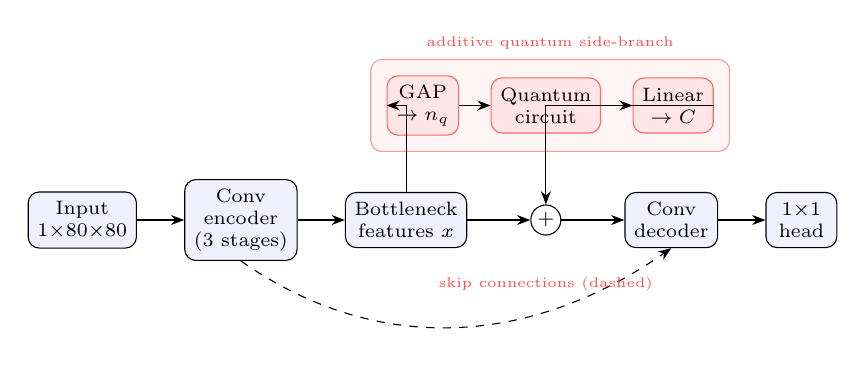
\begin{tikzpicture}[
  font=\scriptsize,
  box/.style={draw,rounded corners,minimum height=7mm,minimum width=9mm,align=center},
  qbox/.style={box,fill=red!10,draw=red!60},
  cbox/.style={box,fill=blue!6},
  >/.tip={Stealth},every edge/.style={draw,-Stealth}
]
\node[cbox] (in) {Input\\$1{\times}80{\times}80$};
\node[cbox,right=6mm of in] (enc) {Conv\\encoder\\(3 stages)};
\node[cbox,right=6mm of enc] (bn) {Bottleneck\\features $x$};
\node[circle,draw,inner sep=1pt,right=8mm of bn] (add) {$+$};
\node[cbox,right=8mm of add] (dec) {Conv\\decoder};
\node[cbox,right=6mm of dec] (head) {$1{\times}1$\\head};
% quantum branch above the (+)
\node[qbox,above=9mm of add] (qc) {Quantum\\circuit};
\node[qbox,left=4mm of qc] (gap) {GAP\\$\to n_q$};
\node[qbox,right=4mm of qc] (po) {Linear\\$\to C$};
\draw (in) edge (enc);
\draw (enc) edge (bn);
\draw (bn) edge (add);
\draw (add) edge (dec);
\draw (dec) edge (head);
\draw[-Stealth] (bn.north) |- (gap.west);
\draw (gap) edge (qc);
\draw (qc) edge (po);
\draw[-Stealth] (po.east) -| (add.north);
\draw[dashed,-Stealth] (enc.south) to[out=-35,in=-145] (dec.south);
\node[font=\tiny,below=4mm of add,red!70] {skip connections (dashed)};
\begin{scope}[on background layer]
\node[draw=red!40,rounded corners,fill=red!4,fit=(gap)(qc)(po),inner sep=2mm,
  label={[red!70,font=\tiny]above:additive quantum side-branch}] {};
\end{scope}
\end{tikzpicture}
\caption{Hybrid quantum--classical architecture. The quantum circuit operates
on a global-average-pooled (GAP) channel vector and its output is broadcast and
\emph{added} to the convolutional bottleneck $x$; it is a global
channel-recalibration side-branch, not a true bottleneck.}
\label{fig:arch}
\end{figure}

\paragraph{Parameter matching.} Classical models auto-select dimension-specific
widths to hold ${\sim}17$M parameters in 2D and 3D. The quantum/hybrid models
use a fixed $3$-stage encoder $[80,160,320]$ giving ${\sim}6.1$M in 2D but
${\sim}17.6$M in 3D ($3$D kernels cost ${\sim}3\times$). The native 2D quantum
models are therefore \emph{not} parameter-matched; we add a second 2D run with
a $4$-stage encoder $[80,160,320,480]\,({=}16.9$M, the ``17M'' variants).

\subsection{Training, metrics and hardware}
Models were trained with Adam~\cite{adam} (lr~$10^{-3}$, cosine schedule,
$5$-epoch warmup), a combined cross-entropy~+~soft-Dice loss~\cite{vnet} with
inverse-frequency class weighting, mixed precision, gradient clipping, and
early stopping (patience~$15$, minimum $250$ epochs) on a single NVIDIA
RTX~3090. We report Dice per foreground class and the mean foreground Dice.
The primary statistical unit is per-subject mean Dice on the six test subjects;
given the small $n$ we report bootstrap $95\%$ CIs of paired differences and
paired Cohen's~$d$ as primary evidence, with Friedman omnibus and
Holm-corrected Wilcoxon tests~\cite{nonparam} as exploratory.

\paragraph{Evaluation protocol.} For 2D training, axial slices with $<20$
foreground voxels are skipped. Applying this filter to the test split scores
\emph{only} brainstem-bearing slices, never penalising false positives on empty
slices and yielding optimistic Dice. We therefore additionally report an
\textbf{honest full-volume 2D evaluation} over all $96$ axial slices per
subject. The 3D models already evaluate whole volumes; consequently 2D and 3D
numbers are not directly comparable. Experiments ran on a workstation with
$2{\times}$RTX~3090 (24\,GB) GPUs (one per run), Python~3.12, PyTorch~2.6,
PennyLane~0.44 and Qiskit~2.4.

% =====================================================================
\section{Results}
All Dice values are per-subject mean~$\pm$~s.d. over the six test subjects.

\subsection{Accuracy at matched capacity}
All architectures achieved high accuracy (Table~\ref{tab:main}). On
foreground-bearing 2D slices the nine matched-capacity models were
statistically indistinguishable (Friedman $\chi^2{=}6.09$, $p{=}0.637$); the
best was a quantum model (Qiskit-QCNN). In 3D the models differed
($\chi^2{=}20.58$, $p{=}0.008$) and the best was classical (MipaimUNet).

\begin{table}[t]
\centering
\caption{Per-subject mean Dice $\pm$ s.d.\ ($n{=}6$). Q=quantum, H=hybrid,
C=classical. 2D shown on foreground-bearing slices at the matched $16.9$M
budget.}
\label{tab:main}
\small
\setlength{\tabcolsep}{4pt}
\begin{tabular}{lcc@{\hskip 1em}lcc}
\toprule
\multicolumn{3}{c}{\textbf{2D (axial slices)}} &
\multicolumn{3}{c}{\textbf{3D (volumes)}}\\
\cmidrule(r){1-3}\cmidrule(l){4-6}
Model & Par. & Dice & Model & Par. & Dice\\
\midrule
Qiskit-QCNN (Q)    & 16.9M & $.932{\pm}.007$ & MipaimUNet (C)     & 17.8M & $.940{\pm}.013$\\
MARIN (C)          & 17.4M & $.932{\pm}.015$ & ACAPULCO (C)       & 17.1M & $.937{\pm}.017$\\
Hybrid-QCNN (H)    & 16.9M & $.932{\pm}.011$ & PennyLane-QCNN (Q) & 17.6M & $.935{\pm}.016$\\
MipaimUNet (C)     & 17.3M & $.931{\pm}.015$ & MARIN (C)          & 17.1M & $.934{\pm}.019$\\
PennyLane-QCNN (Q) & 16.9M & $.930{\pm}.013$ & SwinUNETR (C)      & 17.1M & $.932{\pm}.020$\\
SwinUNETR (C)      & 16.8M & $.929{\pm}.014$ & Hybrid-QCNN (H)    & 17.6M & $.931{\pm}.022$\\
ClassicalCNN (C)   & 17.0M & $.929{\pm}.013$ & CerebNet (C)       & 18.0M & $.930{\pm}.018$\\
ACAPULCO (C)       & 17.4M & $.928{\pm}.017$ & Qiskit-QCNN (Q)    & 17.6M & $.925{\pm}.032$\\
CerebNet (C)       & 16.7M & $.927{\pm}.016$ & ClassicalCNN (C)   & 17.0M & $.920{\pm}.037$\\
\bottomrule
\end{tabular}
\end{table}

\subsection{The quantum bottleneck is the ceiling}
Widening the 2D quantum/hybrid classical encoder from $6.1$M to $16.9$M
parameters produced \emph{no} improvement (PennyLane $\Delta{=}{-}0.0023$,
95\%\,CI $[-0.0046,-0.0005]$; Qiskit $\Delta{=}{-}0.0007$; Hybrid
$\Delta{=}{+}0.0019$; none survived Holm correction). Performance is capped by
the $8$-qubit bottleneck, not the backbone---so the quantum models reach
classical-level Dice with ${\sim}\tfrac13$ of the parameters. The cost is
computational: 2D quantum runs took $8.9$--$13.6$\,h versus $0.3$--$1.0$\,h for
classical models; in 3D the gap narrows (quantum $28$--$35$\,min) as the larger
classical front-end dominates (Fig.~\ref{fig:cost}).

\subsection{Honest full-volume evaluation overturns the 2D result}
Re-scoring the same 2D checkpoints over all $96$ slices per subject changes the
picture substantially (Table~\ref{tab:c2}, Fig.~\ref{fig:c2}). The Friedman
test jumps from $p{=}0.637$ to $\chi^2{=}39.5$, $p{<}0.0001$, and the spread of
mean Dice widens from ${\approx}0.006$ to $0.059$. The filter had masked large
differences in false-positive behaviour on empty slices: MARIN---a co-leader on
filtered slices---falls to \emph{last} ($-0.087$), while the hybrid quantum
models are the most robust. Pooled quantum/hybrid vs classical:
$0.894$ vs $0.878$, $\Delta{=}{+}0.016$, Wilcoxon $p{=}0.031$. The narrow
$6.1$M quantum models show the smallest drops of all.

\begin{table}[t]
\centering
\caption{2D Dice: conventional foreground-only vs honest full-volume
evaluation (per-subject mean, $n{=}6$). $\Delta$ = full-volume $-$ filtered.}
\label{tab:c2}
\setlength{\tabcolsep}{6pt}
\begin{tabular}{llccc}
\toprule
Model & Type & Foreground-only & Full-volume & $\Delta$\\
\midrule
Qiskit-QCNN (17M)    & Q & 0.932 & \textbf{0.905} & $-0.028$\\
CerebNet             & C & 0.927 & 0.899 & $-0.028$\\
ClassicalCNN         & C & 0.929 & 0.898 & $-0.031$\\
Hybrid-QCNN (17M)    & H & 0.932 & 0.898 & $-0.034$\\
SwinUNETR            & C & 0.929 & 0.883 & $-0.046$\\
PennyLane-QCNN (17M) & Q & 0.930 & 0.880 & $-0.050$\\
MipaimUNet           & C & 0.931 & 0.875 & $-0.056$\\
ACAPULCO             & C & 0.928 & 0.866 & $-0.062$\\
MARIN                & C & 0.932 & \textbf{0.845} & $-0.087$\\
\midrule
PennyLane-QCNN (6M)  & Q & 0.932 & 0.914 & $-0.018$\\
Qiskit-QCNN (6M)     & Q & 0.933 & 0.912 & $-0.022$\\
Hybrid-QCNN (6M)     & H & 0.930 & 0.899 & $-0.031$\\
\bottomrule
\end{tabular}
\end{table}

\begin{figure}[t]
\centering
\includegraphics[width=0.78\textwidth]{figures/fig_fullvol_vs_fg_2d.png}
\caption{2D per-subject Dice under foreground-only (grey) vs honest full-volume
(coloured: red = quantum/hybrid, blue = classical) evaluation, sorted by
full-volume score. The filtered metric compresses all models near $0.93$; honest
scoring separates them, with quantum/hybrid most robust.}
\label{fig:c2}
\end{figure}

\begin{figure}[t]
\centering
\includegraphics[width=0.62\textwidth]{figures/fig_cost_2d.png}
\caption{2D accuracy vs training time (log scale). Quantum models occupy the
high-cost region at comparable accuracy, reflecting classical circuit
simulation.}
\label{fig:cost}
\end{figure}

% =====================================================================
\section{Discussion}
At matched capacity, hybrid quantum--classical U-Nets match classical networks
for brainstem subregion segmentation in 2D and trail them slightly in 3D. The
ablation shows their advantage is \emph{parameter efficiency, not accuracy}: an
$8$-qubit bottleneck substitutes for several million convolutional parameters
without loss of Dice, but also caps attainable accuracy; today this is offset
by the cost of statevector simulation.

The more consequential finding is methodological. The conventional
foreground-only 2D protocol made all models look identical, whereas honest
full-volume scoring---which penalises false positives on non-brainstem
slices---separated them by an order of magnitude and reordered the ranking. The
hybrid quantum models, and especially the narrow $6.1$M variants, proved the
most robust, plausibly because the additive global quantum branch acts as a
conservative channel gate that suppresses spurious activations on empty inputs.
This argues that \textbf{brainstem-segmentation benchmarks must be reported on
whole volumes}, not foreground-filtered slices, to be clinically meaningful.
Clinically, every model produced segmentations accurate enough
(medulla/pons Dice ${\sim}0.94$) to support the pontine and medullary atrophy
measurements relevant to SCA2; for deployment a fast classical 3D U-Net remains
the pragmatic choice.

\noindent\textbf{Limitations.} The test set has six subjects, limiting
statistical power; differences are reported as effect sizes with bootstrap
intervals and read as exploratory. Each configuration used a single seed; the
data are single-centre; quantum models were classically simulated. A code audit
also identified a mis-scaled class-weighted Dice term (since corrected); the
reported models were trained with the original loss, so the \emph{relative}
comparison is internally consistent but absolute values may shift after
re-training. Multi-centre cohorts, multi-seed training, full-volume re-training,
and prospective biomarker validation are natural next steps.

% =====================================================================
\section{Conclusion}
On an SCA2-relevant brainstem cohort, parameter-matched quantum and classical
segmentation networks are comparably accurate, with quantum models offering
parameter efficiency at substantial compute cost. Crucially, 2D conclusions
depend on evaluation protocol: honest full-volume scoring reveals hybrid quantum
models as the most robust to empty-slice false positives. The findings support
continued, carefully-controlled investigation of hybrid quantum--classical
segmentation and whole-volume evaluation standards.

\subsubsection*{Acknowledgements.} \todo{Funding and data-collection
acknowledgements.}

% =====================================================================
\begin{thebibliography}{99}
\bibitem{unet} Ronneberger, O., Fischer, P., Brox, T.: U-Net: Convolutional networks for biomedical image segmentation. In: MICCAI (2015)
\bibitem{unet3d} \c{C}i\c{c}ek, \"O., et al.: 3D U-Net: learning dense volumetric segmentation from sparse annotation. In: MICCAI (2016)
\bibitem{vnet} Milletari, F., Navab, N., Ahmadi, S.A.: V-Net: fully convolutional neural networks for volumetric medical image segmentation. In: 3DV (2016)
\bibitem{cerebnet} Faber, J., et al.: CerebNet: a fast and reliable deep-learning pipeline for detailed cerebellum sub-segmentation. NeuroImage (2022)
\bibitem{acapulco} Han, S., Carass, A., et al.: Automatic cerebellum anatomical parcellation using U-Net with locally constrained optimization (ACAPULCO). NeuroImage (2020)
\bibitem{swinunetr} Hatamizadeh, A., et al.: Swin UNETR: Swin transformers for semantic segmentation of brain tumors in MRI images. In: MICCAI BrainLes Workshop (2022)
\bibitem{swin} Liu, Z., et al.: Swin Transformer: hierarchical vision transformer using shifted windows. In: ICCV (2021)
\bibitem{inception} Szegedy, C., et al.: Going deeper with convolutions. In: CVPR (2015)
\bibitem{cbam} Woo, S., Park, J., Lee, J.Y., Kweon, I.S.: CBAM: convolutional block attention module. In: ECCV (2018)
\bibitem{qcnn} Cong, I., Choi, S., Lukin, M.D.: Quantum convolutional neural networks. Nature Physics 15, 1273--1278 (2019)
\bibitem{pennylane} Bergholm, V., et al.: PennyLane: automatic differentiation of hybrid quantum-classical computations. arXiv:1811.04968 (2018)
\bibitem{qiskit} Qiskit contributors: Qiskit: an open-source framework for quantum computing (2023)
\bibitem{n4} Tustison, N.J., et al.: N4ITK: improved N3 bias correction. IEEE TMI 29(6), 1310--1320 (2010)
\bibitem{adam} Kingma, D.P., Ba, J.: Adam: a method for stochastic optimization. In: ICLR (2015)
\bibitem{pulst} Pulst, S.M., et al.: Moderate expansion of a normally biallelic trinucleotide repeat in spinocerebellar ataxia type 2. Nature Genetics 14, 269--276 (1996)
\bibitem{velazquez} Velazquez-Perez, L., Rodriguez-Labrada, R., Fernandez-Ruiz, J.: Spinocerebellar ataxia type 2: clinicogenetic aspects, mechanistic insights, and management. \todo{verify venue/year}
\bibitem{helsinki} World Medical Association: Declaration of Helsinki: ethical principles for medical research involving human subjects. JAMA 310(20), 2191--2194 (2013)
\bibitem{nonparam} Friedman, M.: The use of ranks to avoid the assumption of normality implicit in the analysis of variance. JASA 32, 675--701 (1937); Wilcoxon, F.: Individual comparisons by ranking methods. Biometrics Bulletin 1, 80--83 (1945)
\end{thebibliography}

\end{document}
